\normaltrue
\correctiontrue

%\UPSTIidClasse{11} % 11 sup, 12 spé
%\newcommand{\UPSTIidClasse}{12}

\exer{Mouvement RR  $\star$ \label{B2:13:04:02}}
\setcounter{numques}{0}
\UPSTIcompetence{B2-13}
\index{Compétence B2-13}
\index{Mécanisme à 2 rotations}
\ifcorrection
\else
\textbf{Pas de corrigé pour cet exercice.}
\fi

\ifprof
\else
Soit le mécanisme suivant. On a $\vect{AB}=R\vect{i_1}$ avec $R=\SI{20}{mm}$ et  
$\vect{BC}=L\vect{i_2}$ avec $L=\SI{15}{mm}$.
\begin{center}
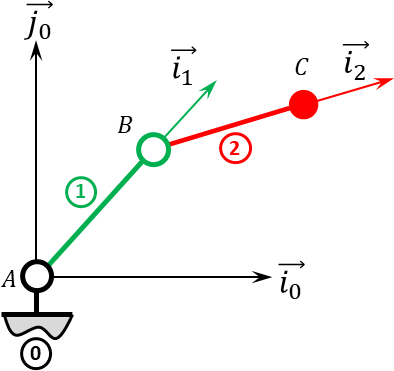
\includegraphics[width=\linewidth]{04_RR_01}
\end{center}
\fi

\question{Déterminer $\vectv{C}{2}{0}$ par dérivation vectorielle.}
\ifprof ~\\
$\vectv{C}{2}{0}$ $ = \deriv{\vect{AC}}{\rep{0}}$
$ = \deriv{\vect{AB}}{\rep{0}}+\deriv{\vect{BC}}{\rep{0}}$
$ = R\deriv{\vect{i_1}}{\rep{0}}+L\deriv{\vect{i_2}}{\rep{0}}$
$ = R\dot{\theta}\vj{1}+L\left( \dot{\theta}+\dot{\varphi}\right)\vj{2}$.

(Avec $\deriv{\vect{i_2}}{\rep{0}} = \deriv{\vect{i_2}}{\rep{2}} + \vecto{2}{0}\wedge \vi{2}$
$ = \left( \dot{\theta}+\dot{\varphi}\right)\vk{0}\wedge \vi{2}$ $ = \left( \dot{\theta}+\dot{\varphi}\right)\vj{2}$).
\else
\fi


\question{Déterminer $\vectv{C}{2}{0}$ par composition.}
\ifprof ~\\
On a $\vectv{C}{2}{0} $ $= \vectv{C}{2}{1}+\vectv{C}{1}{0}$.

$\babarv{C}{B}{2}{1} = -L\vi{2}\wedge \dot{\varphi}\vk{0}= L\dot{\varphi}\vj{2}$.

$\babarv{C}{A}{1}{0} = \left( -L\vi{2} -R\vi{1}\right)\wedge  \dot{\theta}\vk{0}$
$=\dot{\theta}\left( L\vj{2} +R\vj{1}\right)$.

Au final, $\vectv{C}{2}{0} = L\dot{\varphi}\vj{2} + \dot{\theta}\left( L\vj{2} +R\vj{1}\right)$.

\else
\fi

\question{Donner le torseur cinématique $\torseurcin{V}{2}{0}$ au point $C$.}
\ifprof ~\\
$\torseurcin{V}{2}{0}=\torseurcin{V}{2}{1}+\torseurcin{V}{1}{0}$. Pour sommer les torseurs, il faut écrire les vecteurs vitesses au même point, ici en $C$. 

$\torseurcin{V}{2}{0}=\torseurl{ \left( \dot{\theta}+\dot{\varphi}\right)\vk{0}}{R\dot{\theta}\vj{1}+L\left( \dot{\theta}+\dot{\varphi}\right)\vj{2}}{C}$
 \else
\fi

\question{Déterminer $\vectg{C}{2}{0}$.}
\ifprof~\\

$\vectg{C}{2}{0}$ $ = \deriv{\vectv{C}{2}{0}}{\rep{0}}$ $= \deriv{R\dot{\theta}\vj{1}+L\left( \dot{\theta}+\dot{\varphi}\right)\vj{2}}{\rep{0}}$.

De plus,  $\deriv{\vj{1}}{\rep{0}} = \deriv{\vj{1}}{\rep{1}} + \vecto{1}{0}\wedge \vj{1}$
$ =\dot{\theta}\vk{0} \wedge \vj{1} $ $=-\dot{\theta}\vi{1}$ et 
$\deriv{\vect{j_2}}{\rep{0}} = \deriv{\vect{j_2}}{\rep{2}} + \vecto{2}{0}\wedge \vj{2}$
$ = \left( \dot{\theta}+\dot{\varphi}\right)\vk{0}\wedge \vj{2}$ $ = -\left( \dot{\theta}+\dot{\varphi}\right)\vi{2}$.

On a donc $\vectg{C}{2}{0}$ $=R\ddot{\theta}\vj{1}-R\dot{\theta}^2\vi{1}+L\left( \ddot{\theta}+\ddot{\varphi}\right)\vj{2}-L\left( \dot{\theta}+\dot{\varphi}\right)^2\vi{2}$.

\else
\fi

\ifprof
\else
\ifcolle
\else
\footnotesize
\begin{center}
\begin{tabular}{|p{.9\linewidth}|}
\hline
Indications :
\begin{enumerate}
\item $ \vectv{C}{2}{0}= R\dot{\theta}\vj{1}+L\left( \dot{\theta}+\dot{\varphi}\right)\vj{2}$.
\item $\vectv{C}{2}{0} = L\dot{\varphi}\vj{2} + \dot{\theta}\left( L\vj{2} +R\vj{1}\right)$ (c'est la même :)).
\item $\torseurcin{V}{2}{0}=\torseurl{ \left( \dot{\theta}+\dot{\varphi}\right)\vk{0}}{R\dot{\theta}\vj{1}+L\left( \dot{\theta}+\dot{\varphi}\right)\vj{2}}{C}$.
\item $\vectg{C}{2}{0}=R\ddot{\theta}\vj{1}-R\dot{\theta}^2\vi{1}+L\left( \ddot{\theta}+\ddot{\varphi}\right)\vj{2}-L\left( \dot{\theta}+\dot{\varphi}\right)^2\vi{2}$.
\end{enumerate} \\ \hline
\end{tabular}
\end{center}
\normalsize
\fi

\begin{flushright}
\footnotesize{Corrigé  voir \ref{B2:13:04:02}.}
\end{flushright}%
\fi